%Ve vybrané bankovní organizaci analyzujte požadavky na připojení vlastních zařízení a identifikujte hlavní hrozby související s nasazením BYOD.
Tato kapitola seznamuje čtenáře s výsledky analýzy vybrané bankovní organizace. Nejdříve je organizace krátce představena a jsou vyjmenována některá specifika tohoto typu organizací. Dále je podrobně analyzován stávající proces připojování nefiremních zařízení do firemní sítě včetně použitých technických prostředků a tento proces je dále podroben analýze souvisejících hrozeb. V neposlední řadě jsou analyzovány známé požadavky na BYOD dané organizaci a typické skupiny uživatelů a jejich potřeb. Závěr kapitoly se zabývá projekty dotýkajícími se problematiky BYOD, které byly v organizaci uskutečněny již dříve.

\section{Popis vybrané organizace}
Zkoumaná organizace je zadavatelem této diplomové práce. Údaje pro tento popis jsou čerpány z výroční zprávy společnosti pro rok 2016. Jedná se o jednu z největších bank v České republice. Byla založena jako státní organizace, nyní se jedná o akciovou společnost. Majoritní podíl akcií drží mateřská společnost ze zahraničí. Typickým akcionářem je fyzická osoba z České republiky.

Čistý zisk v roce 2016 byl více než 13 miliard Kč, celkové provozní výnosy činily více než 31 miliard Kč, provozní náklady 14 miliard Kč.

Banka má více než 7,5 tisíce zaměstnanců, téměř 400 obchodních míst a více než 1,6 milionu klientů.  

Mateřská společnost je jednou z největších evropských finančních skupin. Působí ve více než 70 zemích, má více než 150 tisíc zaměstnanců a obsluhuje více než 32 milionů klientů. 

\section{Vztah autora práce ke zkoumané organizaci}
Autor této práce v době jejího vypracovávání nebyl zaměstnancem zkoumané organizace. Banka, jako zadavatel této práce, interně vedla autora této práce jako externistu, studenta. Analýza probíhala ve spolupráci s oddělením IT Security. Schůzky a konzultace probíhaly napříč odděleními a byly zprostředkovány oddělením IT Security. 

\section{Specifika bankovního prostředí}
Bankovnictví je specifický obor podnikání, a to především z důvodu vysoké státní regulace. Podle své výroční zprávy se Banka musí řídit mimo jiné následujícími právními předpisy:

\textit{
\begin{itemize}
\item zákon č. 21/1992 Sb., o bankách,
\item zákon č. 256/2004 Sb., o podnikání na kapitálovém trhu,
\item zákon č. 90/2012 Sb., o obchodních korporacích,
\item zákon č. 257/2016 Sb., o spotřebitelském úvěru, (účinný od 1. 12. 2016)
\item zákon č. 284/2009 Sb., o platebním styku,
\item zákon č. 38/2004 Sb., o pojišťovacích zprostředkovatelích a samostatných likvidátorech pojistných událostí a o změně živnostenského zákona,
\item zákon č. 253/2008 Sb., o některých opatřeních proti legalizaci výnosů z trestné činnosti a financování terorismu,
\item zákon č. 69/2006 Sb., o provádění mezinárodních sankcí,
\item zákon č. 563/1991 Sb., o účetnictví,
\item zákon č. 101/2000 Sb., o ochraně osobních údajů,
\item zákon č. 143/2001 Sb., o ochraně hospodářské soutěže,
\item zákon č. 136/2011 Sb., o oběhu bankovek a mincí,
\item zákon č. 190/2004 Sb., o dluhopisech,
\item zákon č. 240/2013 Sb., o investičních společnostech a investičních fondech,
\item zákon č. 89/2012 Sb., občanský zákoník,
\item zákon č. 277/2013 Sb., o směnárenské činnosti,
\item zákon č. 634/1992 Sb., o ochraně spotřebitele,
\item nařízení EU č. 596/2014 o zneužívání trhu,
\item nařízení EU č. 575/2013 o obezřetnostních požadavcích na úvěrové instituce a investiční podniky a navazující prováděcí nařízení Evropské komise,
\item nařízení EU č. 648/2012 o OTC derivátech, ústředních protistranách a registrech obchodních údajů (EMIR).
\end{itemize}
}

Banka, jako provozovatel kritické infrastruktury státu, též spadá pod \textbf{zákon č. 181/2014 Sb. o kybernetické bezpečnosti}, což s sebou mimo jiné nese nutnost reportovat kybernetické incidenty.

Vzhledem k vysoko kladeným nárokům na tento typ společností je nezbytně nutné mít jasně nastavené a kontrolované procesy. Podle výroční zprávy společnosti by z hlediska rizik spojených s nesouladem s regulatorními předpisy znamenalo \textit{naplnění některých z rizik  možné důsledky v podobě vedení sporů s regulatorními orgány, institucemi či klienty, riziko finančních pokut, náhrady škod či nákladů na nápravná opatření a dále riziko ztráty reputace a dobrého jména u klientů i široké veřejnosti, a tím další možné finanční ztráty.}

\subsection{Řízení rizik}
Problematika BYOD spadá pod operační rizika. Banka používá pro řízení operačních rizik přístup AMA -- Advanced Measurement Approach. Při zajišťování informační bezpečnosti vychází z norem ISO/IRC 2700x. Pro řízení rizik se používá nástroj RSA GRC -- Archer.

Hodnocení řízení rizik provádí interní audit


\section{Aktuální stav připojování soukromých zařízení}
Podle aktuální praxe ve zkoumané společnosti je připojení zařízení, které není ve vlastnictví společnosti, a to s ohledem na pracovní informační potřeby pracovníků, možné, ovšem toto je hodnoceno jako nesoulad s dobrou praxí a interními předpisy společnosti. Proto musí být pro každý takový případ udělena bezpečnostní výjimka.

\subsection{Proces udělení bezpečnostní výjimky}
Žádosti o připojování nefiremních zařízení se vyřizují pomocí aplikace Service desk. Jedná se o interní aplikaci vyvinutou a spravovanou uvnitř firmy za účelem řízení IT procesů. Proces pro udělení bezpečností výjimky za účelem připojení zařízení, které není ve vlastnictví společnosti, je ilustrován v diagramu \ref{vyjimka}.

\begin{figure}[h!]
\centering
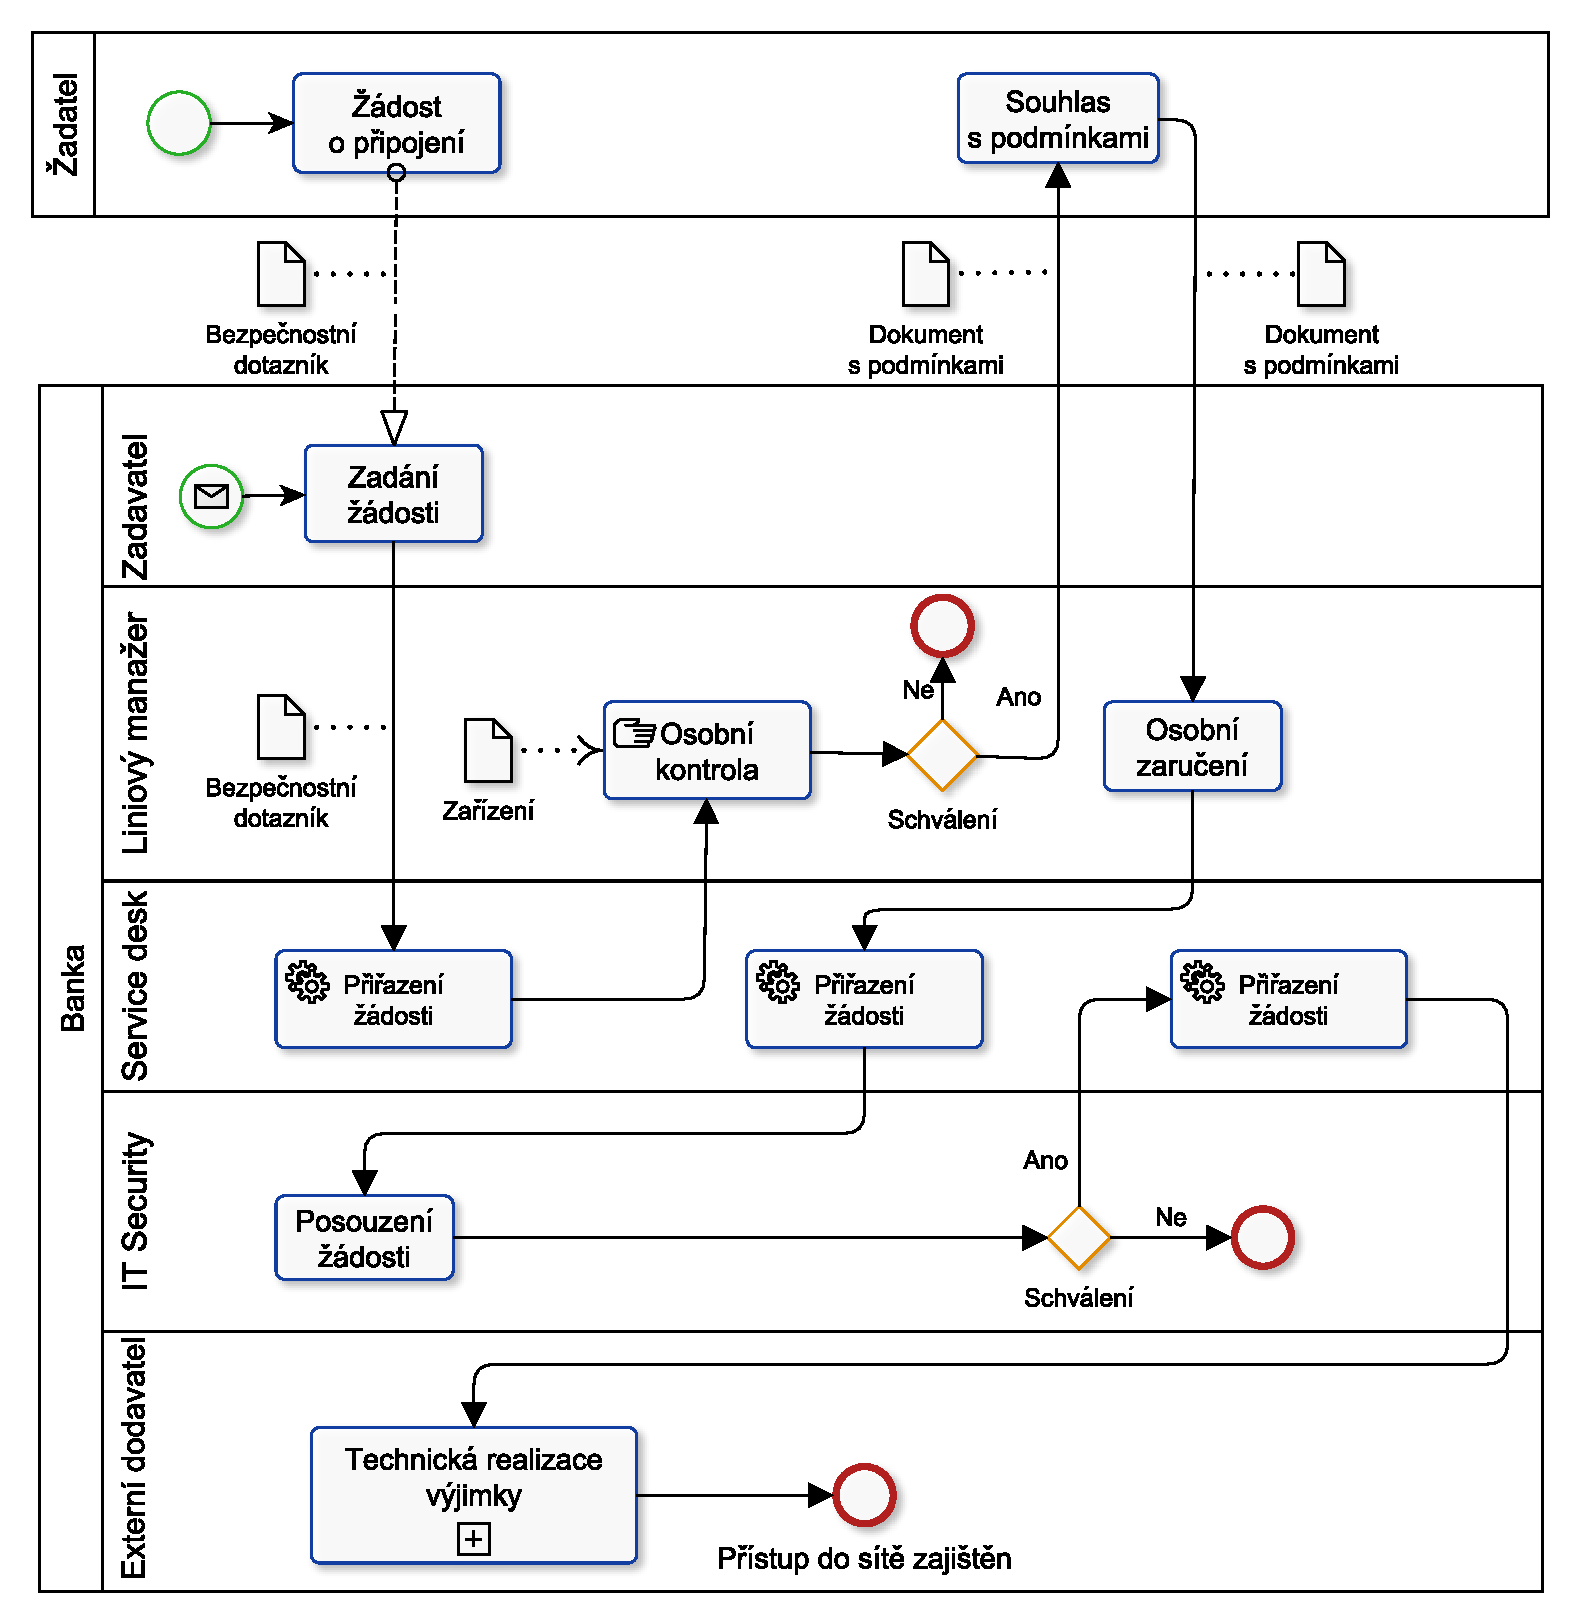
\includegraphics[width=13cm]{img/vyjimkaBPMN}
\caption{Vizualizace procesu pro připojení nefiremního zařízení do vnitřní sítě.\label{vyjimka}} 
\end{figure}

Jelikož žadatel nemá se svým zařízením přístup do vnitřní sítě a tedy ani ke službám aplikace Service desk, je předpokládáno podání žádosti jinou osobou. Jelikož bezpečnostní standardy neumožňují, aby osoba schvalovala vlastní žádost, předkladatelem žádosti nemůže být liniový manažer pod kterého organizačně spadá osoba žadatele. Součástí žádosti je vyplněný bezpečnostní dotazník. 

Dotazník v obecné části obsahuje osobní údaje žadatele, odůvodnění žádosti, typy dat, se kterými bude pracovník nakládat či další informace o vlastnictví zařízení. Technická část dotazuje MAC adresu, použité operační systémy, přítomnost virtualizace, splnění licenčních podmínek software či přítomnost a aktuálnost bezpečnostního software (antivir, firewall, šifrování).

Vytvořený servisní případ žádosti je dále přidělen liniovému manažerovi pod kterého osoba žadatele organizačně spadá. Liniový manažer provede osobní kontrolu zařízení a podepíše se žadatelem dokument specifikující požadavky na žadatele a zařízení. Mezi podmínky patří jednoznačná identifikovatelnost žadatele v rámci informačních systémů společnosti, správnost údajů uvedených v bezpečnostním dotazníku, splnění bezpečnostních politik či splnění licenčních podmínek. Schválením žádosti a jejím postuopením dále se liniový manažer zaručuje za svého podřízeného pracovníka.

Schválenou žádost dále přezkoumá pracovník oddělení IT security. Pokud žádost shledá oprávněnou, předá ji na externí firmu, která udělení bezpečnostní výjimky technicky realizuje. Realizace spočívá ve vytvoření přístupových účtů, přidělení přístupových oprávnění a zadání výjimky pro zařízení do systému spravujícímu přístup do sítě. 

\subsection{Další procesy související s BYOD}
Další procesy jsou buďto triviální, nebo se vymykají rámci této práce a proto nebudou podrobněji analyzovány.

Ve zkoumané organizaci existuje WiFi síť pro hosty.  Je určena především pro návštěvy za účelem obchodních jednání. Přístup k této síti jednoduše vytvoří zaměstnanec Banky ve speciální aplikaci. Pro dlouhodobější vytvoření přístupu zadá zaměstnanec požadavek do systému Service desk.
Připojování nefiremních mobilních zařízení v době psaní této práce nebylo povoleno a tedy neexistoval související proces. Připojování firemních zařízení je mimo rámec této práce. 

\subsection{Připojení z technického hlediska}

Pro správu nefiremních zařízení ve své síti používá zkoumaná společnost nástroj MAB Keeper od společnosti AleFIT. Ta jej v \cite{MABKeeper} definuje následovně: \textit{Aplikace slouží ke správě MAC adres zařízení, která jsou v autentizačním systému použita pro autentizaci, ale nejsou kompatibilní se standardem 802.1x, nebo správě zařízení, u nichž se MAC adresa využívá jako náhradní způsob autentizace. AleFIT MAB Keeper také umožňuje díky několika modulům kontrolovat a časově omezit přístup kontraktorů, konzultantů i BYOD zařízení do firemní sítě, stejně jako využít workflow pro realizaci re-image stanic.} Jedná se o nadstavbu používaného systému Cisco Identity Service Engine (ISE).


Systém ISE řídí nasměrování zařízení do patřičné VLAN na základě adresy MAC. podle příslušnosti k patřičné VLAN má připojené zařízení zajištěna přístupová práva. Ta se řídí pomocí seznamů pro řízení přístupu neboli anglicky Access controll list (ACL). Jedná se tedy o správu připojených zařízení na úrovni topologie sítě. 

Výjimky je možné najít v aplikaci MAB keeper v záložce Approved devices. MAB Keeper tak slouží pro distribuci správy. Mezi používané techniky se řadí MAC address bypass, což znamená obejití standardní autentifikace pomocí protokolu 802.1.X. Jelikož nefiremní zařízení nemají autorizační certifikát, používá se autorizační funkce. Ta zohledňuje MAC adresu a přihlašovací údaje. Uživatelé s vlastními zařízeními a uznanou výjimkou se mohou být přiřazeni do stejné VLAN jako firemní zařízení.


Z hlediska použití bezdrátových sítí WiFi existuje datová síť a síť pro hosty. Pro přístup k datové síti je nutný certifikát, a to především z důvodu fyzické dostupnosti signálu sítě i mimo objekty firemní objekty. Není v plánu další rozšiřování datových WiFi sítí.  

WiFi síť pro hosty je určena pro krátkodobé návštěvníky a umožňuje pouze přístup k síti internet. Důvodem pro její existenci jsou především prezentace obchodních partnerů a další datově méně náročné činnosti. Probíhá na ní URL filtrace.

Jednodenní přístup mohou vytvořit zaměstnanci banky pomocí speciální aplikace. Vytvoření dlouhodobějšího přístupu je možné a vytváří se pomocí žádosti v aplikaci Service desk. 

\section{Cisco ISE}
Společnost Gartner v \cite{GartnerNAC} popisuje Cisco ISE jako jako technologii založenou na protokolu RADIUS. Pokročilé funkce NAC potřebují užitích dalších komponent jako třeba TrustSec Security Group Tag. S použitím device profiling and feed service umožňuje analyzovat provoz a vytvářet reporty o připojených zařízeních.

Balík Cisco AnyConnect sjednocuje další funkce jako jsou VPN, NetFlow nebo ochrana proti škodlivému software. V ISE verze 2.0 je zabudována podpora pro certifikáty, Active Directory či TACACS+.

\section{Analýza aktuálních bezpečnostních rizik spojených s BYOD}
Jelikož metodika analýzy rizik je pro firemního partnera citlivou informací, není pro potřeby této práce možné pracovat s interními metrikami. Vhodné metriky pro hodnocení rizik spojených s kybernetickou bezpečností uvádí zákon o kybernetické bezpečnosti, vyhláška č. 316/2014 Sb., viz \cite{Zakon1}.

Hodnocení rizik používá následující funkci:

$$ riziko = dopad * hrozba * zranitelnost $$


Zákon o kybernetické bezpečnosti udává v § 4, bod (4) vzhledem k bezpečnosti informačních systémů ke zvážení následující hrozby:

\textit{
\begin{enumerate}[label=(\alph*)]
\item porušení bezpečnostní politiky, provedení neoprávněných činností, zneužití oprávnění ze strany uživatelů a administrátorů,
\item poškození nebo selhání technického anebo programového vybavení,
\item zneužití identity fyzické osoby,
\item užívání programového vybavení v rozporu s licenčními podmínkami,
\item kybernetický útok z komunikační sítě,
\item škodlivý kód (například viry, spyware, trojské koně),
\item nedostatky při poskytování služeb informačního systému kritické informační infrastruktury, komunikačního systému kritické informační infrastruktury nebo významného informačního systému,
\item narušení fyzické bezpečnosti,
\item přerušení poskytování služeb elektronických komunikací nebo dodávek elektrické energie,
\item zneužití nebo neoprávněná modifikace údajů,
\item trvale působící hrozby a
\item odcizení nebo poškození aktiva.
\end{enumerate}
}

a dále pak v bodu 6:
\textit{
\begin{enumerate}[label=(\alph*)]
 \item porušení bezpečnostní politiky, provedení neoprávněných činností, zneužití oprávnění ze strany administrátorů kritické informační infrastruktury,
 \item pochybení ze strany zaměstnanců,
 \item zneužití vnitřních prostředků, sabotáž,
 \item dlouhodobé přerušení poskytování služeb elektronických komunikací, dodávky elektrické energie nebo jiných důležitých služeb,
 \item nedostatek zaměstnanců s potřebnou odbornou úrovní,
 \item cílený kybernetický útok pomocí sociálního inženýrství, použití špionážních technik a
 \item zneužití vyměnitelných technických nosičů dat.
\end{enumerate}
}

Zranitelnosti jsou vzhledem k zákonem udávaným typům pro tuto analýzu vzhledem k nastaveným bezpečnostním opatřením pro ochranu informačních systému uvnitř zkoumané společnosti konstantní.

Dále je provedeno hodnocení rizik spojených s připojováním nefiremních zařízení aktuálním postupem pomocí metrik zákona o kybernetické bezpečnosti.

Hrozby e), h), i), j), k) ve vztahu k aktuálně praktikovanému připojování uživatelů s nefiremními zařízeními neexistují, a proto jsou podle stupnice ze \cite{Zakon1} nízké.

Hrozba a) je pravděpodobná, jelikož bezpečnostní politiky není možné vynutit. Hrozbu je tedy nutné hodnotit jako \textbf{střední až vysokou}. Jelikož porušení bezpečnostních politik může mít vliv na chod systémů avšak v omezeném rozsahu a časovém období, lze jej hodnotit jako \textbf{střední}. Výsledné riziko je tedy \textbf{střední až vysoké} a podle použité metodiky by měly být v případě nižší náročnosti zahájeny systematické kroky k jeho odstranění.

Hrozba b) je málo pravděpodobná a její dopad by byl v omezeném období a malého rozsahu. Výsledné riziko je tedy \textbf{nízké}.

Hrozba c) je reálná v případě odcizení zařízení a jeho následném použití pro připojení k firemní síti. Je málo pravděpodobná a nejsou známy žádné případy. Stupeň hrozby je tedy \textbf{střední}. Dopad je v omezeném rozsahu a časovém období, je tedy \textbf{střední}. Riziko je tedy \textbf{střední} a je tolerovatelné pouze pokud by protiopatření byla vyšší náročnosti.

Hrozba d) je pravděpodobná jelikož není možné kontrolovat veškerý nainstalovaný software na zařízení a shodu licenčního ujednání s firemními podmínkami. Stupeň hrozby je tedy \textbf{střední až vysoký}. Jelikož pracovník se smluvně zavázal, že nelicencovaný software používat nebude, břímě odpovědnosti leží na jeho osobě. Případné dopady tedy mohou být přeneseny na něj a hodnocení dopadů je tak \textbf{nízké}. Výsledné riziko je tedy \textbf{nízké až střední}.

Hrozba f) je spíše pravděpodobná. Přestože se uživatel zavázal k používání zazáplatovaného systému a aktuální antivirové ochrany, není možné toto vynutit a monitorovat bezpečné chování uživatele. Tuto hrozbu je možné hodnotit jako \textbf{střední až vysokou}. Teoretický dopad může být nezanedbatelného rozsahu a způsobit škodu. Riziko je tedy \textbf{střední až vysoké} a měly by být zahájeny kroky k jeho odstranění.

Hrozba l) je reálná, stávající opatření nijak neznesnadňují případnému pachateli odcizení aktiv, předpokládaná realizace hrozby však není častá a lze ji proto hodnotit jako \textbf{nízkou až střední}. Finanční ztráty by mohly být znatelné, avšak rozsah dopadu se zdá být omezený, dopad tak lze hodnotit jako \textbf{nízký} a celkové riziko jako \textbf{nízké až střední}.

Vzhledem k dalším uvedeným hrozbám lze konstatovat, že připojování nefiremních zařízení na základě výjimek oproti firemním zařízením znamená zvýšení pravděpodobnosti hrozby c), f) a g), a proto je třeba jim věnovat pozornost. 

\subsection{Zhodnocení analýzy rizik}\label{analyzaRizik}
Při porovnání s užitím firemního zařízení byla při stávajícím způsobu připojování nefiremního zařízení identifikována zvýšená pravděpodobnost realizace některých hrozeb potažmo rizik. Tato práce si klade za cíl hodnotit možná řešení především z hlediska bezpečnosti a navrhnout tak řešení, která identifikovaná rizika zásadním způsobem sníží.

\subsection{Analýza hrozeb souvisejících s nasazením BYOD}
Jelikož BYOD zařízení již nyní ve firemní síti existují, nasazení navrhovaného BYOD programu nijak nezvyšuje pravděpodobnost žádné ze známých hrozeb. V této práci navrhované řešení se soustředí na bezpečnost a tedy nejenom že nezvyšuje pravděpodobnost realizace známých bezpečnostních hrozeb oproti stávajícím firemním zařízením, ale naopak zvyšuje bezpečnost oproti aktuálnímu způsobu připojování nefiremních zařízení.


\section{Analýza požadavků na připojení vlastních zařízení} 
Formou konzultací se zaměstnanci zkoumané společnosti napříč různými odděleními bylo identifikováno několik požadavků a potřeb.

\subsection{Obecné požadavky}\label{obecnePozadavky}

Jedním z hlavních požadavků je přiměřenost z hlediska nákladů. Návrh řešení je třeba obhájit před vedením společnosti, které schvaluje rozpočty projektů. Zároveň je žádoucí, aby řešení mělo kladné přijetí od potencionálních uživatelů, tak aby byli ochotni jej využívat a náklady na zavedení nebyly vynaloženy zbytečně.  

Smyslem vytvoření BYOD programu je vytvoření uceleného návrhu, který umožní zaměstnancům v odůvodněných případech využívat vlastní zařízení a především zvýší bezpečnost existujících BYOD, které se nyní objevují převážně u kontraktorů. Existující riziko, plynoucí z nespravovaných nefiremních zařízení v síti, je třeba potlačit, což je nejsilnějším argumentem pro prosazení projektu.

Důvody k zavedenní řešení BYOD lze tedy rozdělit na technologicko-sociální a obchodní. Je zřejmé, že vzhledem k nastoleným trendům je nutné nastolit firemní strategii pro BYOD. Pokud by se řešení nenašlo, nefiremní zařízení se přesto budou rozšiřovat, ovšem nebudou pod kontrolou firemního IT oddělení. To v důsledku znamená, že nebude možné kontrolovat rizika ani náklady s tímto spojené. 

Z pohledu oddělení IT Security je majoritním důvodem pro řešení otázky BYOD aktuální stav, kdy jsou nefiremní zařízení připojována na základě bezpečnostních výjimek. Tento stav je nežádoucí a je identifikován jasný požadavek pro nastolení rámce, který eliminuje hrozby z toho plynoucí.


\subsection{Identifikované potřeby}\label{identifikovanePotreby}
\begin{itemize}
    \item Tablety pro vrcholový management
    \item Vlastní notebooky
    \item Vlastní počítače Apple
    \item Firemní notebooky externích konzultantů
    \item Přístup k dokumentům ze soukromých tabletů
    \item Přístup k emailu či kalendáři z osobního chytrého telefonu
\end{itemize}

\subsection{Identifikované služby}\label{identifikovaneSluyby}
Z hlediska souvisejících služeb poskytovaných IT byly identifikovány služby typu \textbf{PIM}\footnote{Personal Information Management} neboli služby pro správu osobních informací, typicky se jedná o kalendář, email a další komunikační a organizační systémy, jimiž jsou například Oultook a Skype for Bussiness. Dále je třeba zprostředkovat služby pro \textbf{tvorbu a sdílení dokumentů}. Typicky se jedná o Microsoft Office či Atlassian Confluence. V neposlední řadě je nutný přístup k \textbf{business aplikacím}.

\subsection{Identifikované typy zařízení}
Co se týče různých typů zařízení, je třeba do BYOD programu zařadit firemní chytré telefony včetně zařízení BlackBerry a tablety. Co se týče nefiremních či osobních zařízení je třeba zohlednit chytré telefony, tablety, notebooky či notebooky od firmy Apple.

\subsection{Identifikovaní uživatelé}
Jako uživatelé byli identifikováni zaměstnanci Banky, externí dodavatelé, kontraktoři a klienti.

Skupinou uživatelů, která z principu přichází s vlastními zařízeními jsou externisté, jež Banka z pravidla najímá pro účely projektů. Tito uživatelé můžou pracovat na živnostenský list, nebo mohou být zaměstnanci externího dodavatele. Uživatelé pracující na živnostenský list používají zpravidla soukromá zařízení, zaměstnanci externích dodavatelů používají zpravidla zařízení ve vlastnictví a správě svého zaměstnavatele.

Jako nejčastější typy pracovníků z externích zdrojů byli identifikováni:
\begin{itemize}
    \item Projektoví manažeři
    \item Vývojáři
    \item IT konzultanti
\end{itemize}

Projektoví manažeři jsou zpravidla najímáni pro své know-how z jiných projektů. Mezi priority v jejich potřebách patří firemní služby typu PIM (kalendář, email,\ldots) nástroje pro vytváření dokumentů a kolaboraci, přístup k dokumentům a datům či další nástroje potřebné k řízení projektů. 

IT konzultanti potřebují používat nástroje, dokumenty a služby spojené s danou konzultační činností, kterou Bance poskytují. Problematika vývojářů je popsána v odstavci \ref{potreby_vyvojar}.

V případě externích pracovníků je obzvláště nutné dbát na ochranu firemních dat. Je užitečné mít možnost zajistit, že po ukončení své činnosti tito pracovníci dále nebudou moci nakládat s firemními aktivy. Tito pracovníci se musí řídit vnitřními směrnicemi banky. V případě bezpečnostního incidentu je možné tyto pracovníky nebo jejich zaměstnavatele právně postihovat, typicky pokutou, a to na základě standardně uzavíraného právního vztahu.

Zájem o používání vlastních zařízení však mají i zaměstnanci Banky. Identifikováni byli především uživatelé z vedení společnosti (počítače Mac, tablety iPad) a vývojáři. Pokud se vinou svého vlastního zařízení dopustí bezpečnostního incidentu zaměstnanec banky, je jeho zodpovědnost obtížněji vymahatelná.

\subsection{Způsoby připojení k síti}
Z hlediska připojení k síti byly identifikovány následující možnosti: připojení do sítě LAN, připojení do lokální WiFi a připojení skrze síť internet a mobilní připojení.

\subsection{Způsob podpory od IT oddělení}
Momentálně IT oddělení poskytuje end-to-end podporu. To znamená, že dodaní služeb je podporováno kompletně od zdroje, přes dodání po podporu koncových zařízení. Tento model není trvale udržitelný pro BYOD, kdy není možné podporovat všechna koncová zařízení a je tedy třeba zavést i model, kde je podporována pouze samotná služba. Návrh způsobu podpory pro BYOD je rozveden v kapitole \ref{dalsi_opatreni}.

\subsection{Identifikace potřeb specifického uživatele -- vývojáře}\label{potreby_vyvojar}
Vývojáři patří mezi prioritní skupinu uživatelů, pro které je třeba připravit projekt BYOD. Právě mezi vývojáři je velké množství kontraktorů, kteří si přinášejí své vlastní nefiremní zařízení. Vývojáři však mají vyšší požadavky než běžní uživatelé. Konzultací se zástupci vývojářů v Komerční bance byly identifikovány následující potřeby. 

Vývojář potřebuje mít na zařízení, na kterém vyvíjí, administrátorská oprávnění. Je to především z důvodu instalace pomocných nástrojů, tak z důvodu přístupu k některým systémovým funkcím operačního systému, například pro potřeby testování. Dále má vývojář zvýšené nároky na výpočetní výkon stroje, na kterém němž pracuje, především z důvodu potřeby lokální kompilace zdrojových kódů. 

Vývojáři mají specifické požadavky na nainstalované aplikace. Každý potřebuje vývojové prostředí (Banka nemá sjednoceno, a tedy vývojáři mohou volit nástroj dle svého uvážení, například IntelliJ Idea). Poté jsou to nástroje pro vývoj databází, například Oracle SQL Developer. Dále je nutné přistupovat k dalším databázím. V prostředí zkoumané organizace se používají různé databáze (Oracle, MySQL, MS SQL). Mezi dalšími nezbytnými nástroji byl uveden SSH klient Putty.

Byla zmíněna potřeba přístupu k následujícím službám:
\begin{itemize}
    \item Přihlašování do domény
    \item Přístup k logům -- k centrálnímu systému logů na systému Logman
    \item Přístup k nástroji pro zpracování výstupních streamů Apache Kafka
    \item Přístup k verzovacímu systém GIT na platformě BitBucket
    \item Přístup k systému pro evidenci chyb Atlassian JIRA
    \item Přístup k nástroji pro dokumentaci Atlassian Confluence
    \item Přístup k nástroji pro automatizaci správy software Jenkins
    \item Přístup k testovacím prostředím
    \item Přístup k emailům 
    \item Přístup ke službě Skype for business
    \item Přístup k adresářové službě LDAP
    \item Přístup ke správě identit ITIM
\end{itemize}

Pokud se vývojář připojuje vzdáleně, klade důraz na přístup k verzovacíu systému GIT, přístup k testovacímu prostředí a přístup k logům.

\section{Aktuální stav podpory různých typů zařízení dle typu vlastnictví}


Nejvyšší prioritou je umožnit uživatelům se soukromými zařízeními plný a kontrolovaný přístup ke službám lokální sítě. Není nutné zajišťovat vzdálený přístup pro nefiremní zařízení, je však třeba podporovat vzdálený přístup k emailu. Pro mobilní telefony je třeba zajistit přístup k emailu. Přístup k dokumentům a aplikacím zatím není vyžadován. Byl identifikován požadavek na firemní tablety od vrcholového managementu. Pro ty je třeba zajistit maximální přístup. Uživatelé soukromých tabletů požadují přístup k emailu a dokumentům.

% Please add the following required packages to your document preamble:
% \usepackage{multirow}
\begin{table}[]

\centering

\resizebox{\textwidth}{!}{\begin{tabular}{c|l|l|l|l}
 &  & firemní zařízení & Soukromé zařízení & Zařízení kontraktora \\ \hline
\multirow{2}{*}{Notebook} & Lokálně & Dostupné & Nepodporované ale používané & \multicolumn{1}{l}{Nepodporované ale používané} \\ %\cline{2-5} 
 & Vzdáleně & Dostupné přes VPN & Nepodporované & \multicolumn{1}{l}{Nepodporované} \\ \hline
\multirow{2}{*}{Tablet} & Lokálně & Nedostupné & Nedostupné & \multicolumn{1}{l}{Nedostupné} \\ %\cline{2-5} 
 & Vzdáleně & Nedostupné & Nedostupné & \multicolumn{1}{l}{Nedostupné} \\ \hline
Chytrý telefon & Vzdáleně & Dostupné pro BlackBerry & Nedostupné & \multicolumn{1}{l}{Nedostupné} \\ %\cline{1-1}
\end{tabular}}

\caption{Tabulka aktuálního stavu podpory pro jednotlivé typy zařízení podle typu vlastnictví}
\label{tabulka1}

\end{table}
%\todo{tabulka}


\section{Předešlé projekty}
Projekt na vyhodnocení konceptu BYOD byl v bance započat již v roce 2013. Měl za cíl vyhodnotit rámec pro konkrétní potřeby, scénáře a služby, dále měly být nastaveny předpokládané výstupy a definováno možné řešení. Již v roce 2013 byl citelný příklon uživatelů ke konzumerizaci informačních technologií a prorůstání jiných než-li PC zařízení do firemního prostředí.

V té době se mobilní připojení stalo standardem i pro běžné uživatele a ti tak byli neustále připojeni se svými osobními zařízeními k internetu. Dále byla citelná osobní potřeba zaměstnanců používat svá osobní zařízení i během pracovní doby.

Projekt nastolil možnost zpřístupnění přístupu k emailu i z nefiremních zařízení. Důvodem je zvýšení pracovní efektivity při minimálních dodatečných výdajích. Na mnohých pracovních pozicích by též zavedení BYOD programu umožňovalo flexibilnější pracovní styl. S tím souvisí i snadnější přístup ke klientům. 
Flexibilnější přístup umožňuje lépe uplatňovat techniky křížného prodeje\footnote{Křížný prodej, někdy též křížový prodej (anglicky cross-selling), je obchodní taktika navyšování prodeje, jejímž cílem je prodat více, doporučením souvisejícího zboží nebo služeb, viz \cite{ManagementMania}}. Bezprostřední přístup k informacím by znamenal rychlejší reakci obchodníků a konkurenční výhodu. 

\subsection{Dříve zvažované možnosti pro email}
V minulosti bylo zvažováno několik možností, jak zpřístupnit email a dokumenty na soukromých chytrých telefonech a tabletech.

Exchange ActiveSync snižuje riziko krádeže díky vynucení zadání PIN kódu a možnosti vzdáleného smazání. V jeho prospěch hrála relativně snadná a rychlá implementace. Řešení bylo zamítnuto, protože nenabízelo zašifrování dat. To může znamenat ohrožení dat například při jail-breaku u zařízení iPhone.

V rámci mateřské skupiny se používá řešení Good mail (nyní BlackBerry Work). Toto řešení nevyhovovalo požadavkům vzhledem k vysokým nákladům na implementaci a provoz. Nicméně projekt pro toto řešení stále existuje.

Microsoft Outlook Web App umožňuje prohlížení příloh přímo na serveru a není tedy nutné lokální šifrování dat. Řešení je vhodné jak pro mobilní zařízení, tak tablety a nepřináší žádné dodatečné náklady, jelikož je již implementováno. Uživatelé však nehodnotí uživatelskou přívětivost tohoto řešení příliš kladně.

\subsection{Projekt VDI pro vývojáře a testery}\label{projektVDI}

V Bance též existoval projekt, který se snažil ověřit možnost využití virtuálních strojů pro vývojáře a testery. Důvodem byla snaha získat řešení pro vlastní zařízení kontraktorů, která znamenají bezpečnostní riziko. Dále si Banka od projektu slibovala nalezení řešení problému s využíváním několika zařízení vývojáři, ať už z důvodu vzdálené podpory nebo zvláštních požadavků na výkon.

Test VDI se odehrál v roce 2011, probíhal tři týdny a zúčastnilo se ho 5 vývojářů. Uživatelé po dobu testu prováděli veškeré své pracovní úkony ve virtuálním prostředí. Virtuální stroje běžely na serveru Proliant DL380 G5 s parametry: 4x (2CPUx2jádra) CPU 3000MHz, 24GB RAM a 1,3TB místa na disku. Parametry pro jednotlivé virtuální stroje byly ekvivalentí k PC dvoujádrovým procesorem a 2-4 GB RAM.

Účastníci testu ohodnotili uživatelský zážitek jako dostatečný pro běžné použití. Zaznamenali však nižší odezvu a občasné záseky. Byly identifikovány problémy s periferními zařízeními, například nefungovala čtečka na čipové karty. Odezva vývojářských nástrojů byla odhadem dvakrát pomalejší. Uživatelé hodnotili přechod k virtuálním strojům jako zhoršení uživatelského komfortu oproti fyzickým firemním PC. 

Test prokázal vysoké nároky na diskové úložiště především co se týče počtu požadavků na vstupně/výstupní operace. To znamená nutnost vysoké investice do kvalitního diskového úložiště. Zároveň je nutné zajistit kvalitní konektivitu. Proto bylo rozhodnuto, že VDI není vhodné pro interní vývojáře, protože zvyšuje náklady a nepřináší benefity.

Zároveň test doporučil ke zvážení zkoušený model VDI pro kontraktory, a to pod podmínkou užití vlastního zařízení bez dalších nákladů pro Banku, bez zajištění vysoké dostupnosti a omezení velikosti diskové kapacity pro virtuální stroje na odhadovaných 70-80GB.